\documentclass[10pt,a4paper]{article}

\usepackage[a4paper,top=17mm,bottom=18mm,left=20mm,right=20mm]{geometry}
\usepackage{microtype}
\usepackage{graphicx}
\usepackage{booktabs}
\usepackage{tabularx}
\usepackage{array}
\usepackage{enumitem}
\usepackage{amsmath}
\usepackage{xcolor}
\usepackage{fancyhdr}
\usepackage{float}
\usepackage[hidelinks]{hyperref}

\definecolor{RuleGray}{gray}{0.75}

\setlength{\parindent}{0pt}
\setlength{\parskip}{4pt}
\setlist[itemize]{leftmargin=5mm,itemsep=1pt,topsep=2pt}
\renewcommand{\arraystretch}{1.12}
\renewcommand{\figurename}{Figure}
\renewcommand{\tablename}{Table}

\pagestyle{fancy}
\fancyhf{}
\fancyhead[L]{\small INFO4271 Modern Search Engines}
\fancyhead[R]{\small Group Project Report}
\fancyfoot[C]{\small\thepage}
\renewcommand{\headrulewidth}{0.4pt}
\renewcommand{\footrulewidth}{0pt}
\setlength{\headheight}{13pt}

\begin{document}

\begin{center}
  {\Large\bfseries BeMaMaJa}\\[3pt]
  {\normalsize Group Project Report -- INFO4271 Modern Search Engines}\\[7pt]
  \textbf{Matthias Vetter, Marcel John, Janis Weller, Bernhard Fraidel}\\[2pt]
  \url{https://github.com/BeMaMaJa-Search-Engine/BeMaMaJa-Search-Engine.git}
\end{center}

\begin{abstract}
  This project presents a search engine built from scratch for English-language web pages related to T\"ubingen. It starts with a web crawler that uses a given seed set to retrieve web pages.
To avoid crawling undesirable websites, a blacklist is used, and the crawler respects the robots.txt protocol. To improve performance, the crawler uses multiple worker threads.
For indexing, the retrieved pages are tokenized, stopwords are removed, and the remaining words are stemmed before constructing the inverted index.
The retrieval stage is based on the BM25 algorithm with an integrated spelling correction mechanism. For re-ranking,
we combine the BM25 score with field boosts, link counts, PRF, location-aware ranking signals, and soft domain diversification.
The frontend provides a modern interface with controllable AI-generated page summaries,
explainable ranking signals and direct batch-file upload.
\end{abstract}

\section{Data Collection and Crawling}
  \subsection{Corpus scope and seeds}
  Our corpus contains English-language websites related to Tübingen. For the initial seed
  set, we selected around 50 keywords covering attractions, the university, student life,
  hospitals, culture, and other city topics. For each keyword, we searched Google for
  ``Tübingen + keyword'' and manually recorded the first ten results. Removing duplicate
  URLs left 449 unique seeds. We then added \href{https://scells.me/}{https://scells.me/}
  manually, bringing the final seed set to 450 URLs. The broad range of keywords was intended
  to produce a diverse corpus rather than focusing only on the most common tourist pages.

  \subsection{Crawler design}
  We implemented four crawler versions and evaluated each for about 15 hours under the same
  conditions before selecting the best-performing version for the final crawl. Version 1 followed
  the architecture from the lecture. It used a prioritized frontier, crawl delays, a custom user
  agent, and multiple worker threads. It also respected blocked paths and crawl delays from
  \texttt{robots.txt}, while caching each file to avoid repeated downloads. We used
  \texttt{langdetect} instead of website-provided language metadata. Duplicate content was kept
  during crawling and removed during preprocessing. This increased the size of
  \texttt{raw\_pages.json} but avoided slowing down the crawler.

  Version 2 retained this design but expanded the regular expression for Tübingen-related
  pages to cover spelling variations and OCR-like errors such as ``Tueeebingen'' and
  ``t123bingen''. This allowed relevant pages to be detected even when the city name was
  misspelled or written in an unusual style.

  Version 3 addressed the increasing cost of sorting a large global frontier, which often blocked
  the worker threads. It split links into a high-priority frontier for links from Tübingen-related
  pages and a low-priority frontier for links from unrelated pages. Instead of one large URL data
  structure, each frontier stored domain objects with a queue of URLs and the last access time.
  The crawler randomly selected a ready domain and processed its next URL in discovery order.
  Ready domains had an equal chance of being selected regardless of queue size, so a large website
  with thousands of links could not dominate a smaller domain. Selection depended on the number
  of domains rather than the total number of URLs, which kept frontier operations efficient even
  when millions of links were stored. This also allowed the main thread to spend less time managing
  the frontier and more time supplying work to the workers. The trade-off was losing fine-grained
  prioritization within a domain: a URL containing ``Tübingen'' could be processed after less
  relevant URLs from the same website. However, Version 3 still crawled roughly four to five times
  as many pages as Versions 1 and 2.

  Version 4 added two worker types. Horses selected a random ready domain as before, while
  Explorers preferred ready domains with only a few URLs left. Since Horses would eventually
  reach these domains as well, this was expected to have little effect on overall throughput.
  Its purpose was to discover new domains slightly earlier and improve exploration. We also
  maintained a domain blacklist containing \href{https://archive.org}{https://archive.org}.

  \subsection{Results}
  We evaluated the crawlers with \textit{scripts/crawler\_analysis.py}. After about ten hours,
  Versions 1 and 2 still found the most unique domains, whereas the later versions achieved
  almost four times the page throughput. Comparing Versions 2 and 4, Version 4 collected about
  3.57 times as many pages while finding about 4\% fewer domains. We accepted this trade-off,
  especially because the globally sorted frontier of Versions 1 and 2 became slower as it grew.

  \begin{table}[H]
    \centering
    \small
    \begin{tabular}{lrrrr}
      \toprule
      \textbf{Crawler} & \textbf{Runtime (min)} & \textbf{Domains} & \textbf{Raw pages} & \textbf{Pages/min} \\
      \midrule
      Base (V1, blue) & 632 & 471 & 5187 & 8.21 \\
      Regex (V2, orange) & 583 & 484 & 5201 & 8.92 \\
      Harsh Frontier (V3, red) & 635 & 416 & 20001 & 31.50 \\
      Horses \& Explorers (V4, purple) & 628 & 452 & 20000 & 31.85 \\
      \bottomrule
    \end{tabular}
    \caption{Crawler version comparison after about ten hours.}
  \end{table}

  \begin{figure}[H]
    \centering
    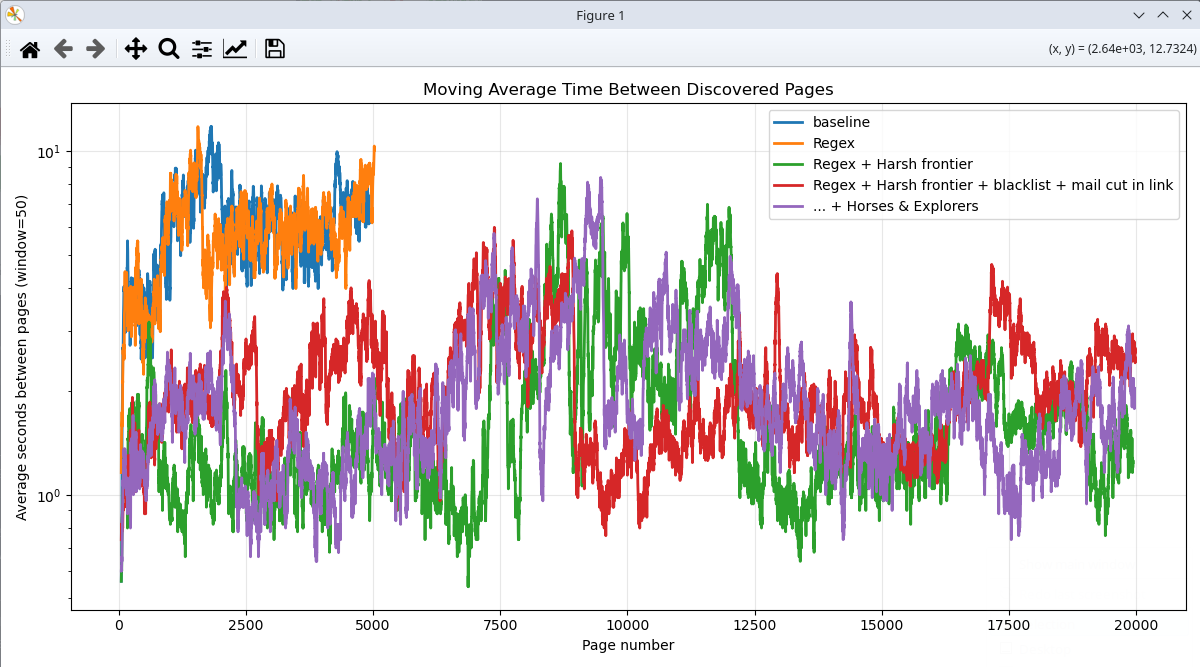
\includegraphics[height=40mm]{img/mse_crawler_1.png}\hfill
    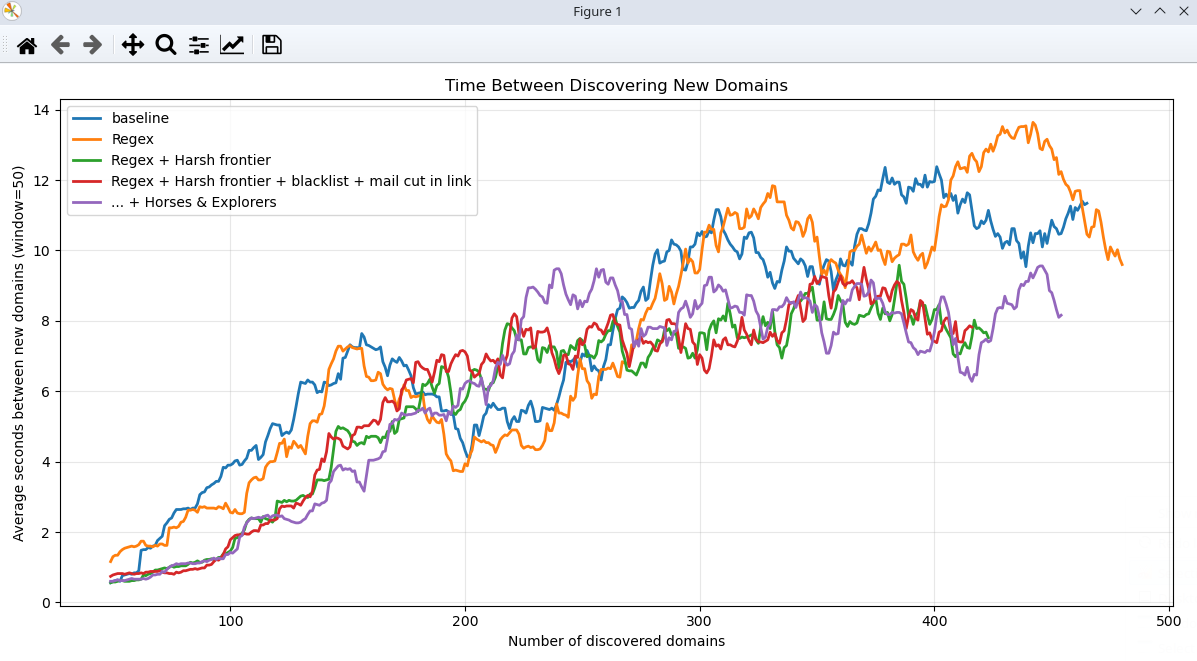
\includegraphics[height=40mm]{img/mse_crawler_2.png}
    \caption{Crawler analysis using a sliding window of 50: average time between finding new pages (left), and time between discovering new domains with the total number of domains found (right). Lower is better.}
  \end{figure}

\section{Preprocessing and Index Construction}
After crawling, exact and near-duplicate pages were removed, reducing the dataset by approximately
30\%. Clearly non-English pages were filtered using language detection and a separate check for
pages in which at least 25\% of the alphabetic characters were non-Latin. Title, headings, and body
were processed separately. The text was lowercased, Unicode accents and different spellings of
  Tübingen were normalized, and it was then tokenized. Finally, stopwords were removed and Porter
stemming was applied. Queries use the same preprocessing pipeline.

The processed documents were used to construct the inverted index. We also stored document
frequencies, field lengths, and the average document length. An internal link graph was built to
support link-based re-ranking in later stages.

\section{Retrieval and Re-ranking}

\subsection{Manual BM25 first stage}
BM25 is used for first-stage ranking because it is a standard algorithm in practice.
It computes the Inverse Document Frequency (IDF) to give rare words a higher value.
Since the search engine is T\"ubingen-based, the IDF for T\"ubingen is boosted by a factor of $2$.
The Term Frequency (TF) is used to give words that appear more often a higher value. 
The final BM25 score is obtained by summing the contribution of each query term.
The parameter $b$ controls the strength of the document length normalization.
The value $b = 0.75$ is chosen since it is the default value in the literature.
The parameter $k_1$ controls the rate of term saturation. Here, the value $k_1 = 1.2$ is chosen since it is the default value in the literature.
\cite{robertson2009bm25}

\subsection{Query processing}
For BM25 and spelling correction, the existing cache is used to load the JSON file.
The file contains the documents and their vocabulary. This vocabulary is separated into buckets for
later spelling correction. Using the cache provides a significant speedup because the JSON file is loaded and parsed only once.
Once the data is loaded, the query tokens are preprocessed in the same way as the indexed documents. The spelling
of each query term is then checked. The algorithm first checks whether the term exists in the vocabulary, which is built
from the indexed pages and contains stemmed terms. If it exists, the spelling is considered correct and
no correction is needed. Otherwise, the term is treated as a possible spelling mistake, and the
algorithm tries to correct it.
To avoid changing a word too much, at most one character can be changed in words shorter than five characters and at most two in longer words.
The buckets are sorted by first letter and word length, so only suitable candidates have to be evaluated.
For further speedup, the algorithm exits early if it is no longer possible to find a better term.
Next, the Levenshtein edit distance \cite{levenshtein1966} is computed to measure how similar two words are.
This is used to find the best candidate. If two words have the same edit distance, their frequency is used as a tie-breaker,
since the assumption is that a user is more likely to search for a more frequently used term. If the edit distance for the best candidate
is above the number of characters that are allowed to be changed, the word will not be changed to avoid changing the query too much.
After a term has been corrected, the word is stemmed again to ensure the resulting term is the same as without the spelling mistake,
thus the search results are also identical.
After this, the BM25 score is computed, and the result is then used by the reranking algorithm.

\subsection{Second-stage innovation}
As second-stage innovations, we use multiple signals to rerank our results.
The final score is a weighted sum of all these components. 
($0.60$ BM25, $0.20$ Field Boost, $0.10$ Link Score, $0.05$ PRF, $0.05$ Tuebingen Centrality, $-0.10$ Location Penalty)

\textbf{Field Boost} increases the score when query terms appear in the title or the headings. 
Matches in these fields are generally stronger relevance indicators than occurrences in the body.
For the computation, the following formulas are used,
where $Q$ is the query tokens, $T$ represents the title tokens, and $H$ represents the heading tokens.
\[
\mathrm{TitleCoverage} =
\frac{|Q \cap T|}{|Q|}
\]
\[
\mathrm{HeadingCoverage} =
\frac{|Q \cap H|}{|Q|}
\]
\[
\mathrm{FieldBoost} =
0.7 \cdot \mathrm{TitleCoverage}
+
0.3 \cdot \mathrm{HeadingCoverage}
\]

\textbf{PRF} is performed by taking the first 30 BM25 candidates. 
Only the strongest from each domain is considered. Up to 5 documents are selected.
Terms are collected from the titles and headings of these five documents.
Query terms, generic terms, and terms that are too rare or too frequent in the corpus are removed.
At most three expansion terms are retained.

\textbf{Link Score} represents the authority of a document within the crawled collection. 
It is defined as the number of indexed documents that link to the candidate.

\textbf{Tübingen Centrality} measures how strongly a document is focused on Tübingen. 
It is based on the occurrence of the normalized "tubingen" term in important document fields.

\textbf{Foreign Location Penalty} reduces the score of documents that appear to focus on another city, such as Stuttgart, Munich, Heidelberg, or Freiburg.
The penalty depends on where the foreign location occurs. Matches in the title receive the strongest penalty, followed by headings and the URL.

\subsection{Domain diversification}
To prevent the result list from being dominated by a single website, we added a soft
domain-diversification step after reranking. The first result from each domain keeps
its full score. Further results from the same domain are progressively penalized using
a factor of $0.93$ per repetition. The penalty is limited to a minimum factor of $0.75$.
We intentionally avoided a strict domain limit because several pages from the same
website may still be highly relevant. This approach improves result variety while
ensuring that relevant documents remain within the top 100 results used for evaluation.


\section{Frontend and Hosting}

\textbf{Frontend innovations.} A good search engine should not only return relevant 
links, but also help users understand and work with the results. This is why we 
added several helpful innovations, mainly focused on controllable AI summaries for 
individual pages and clear insight into why each result appears at its position.

\begin{center}
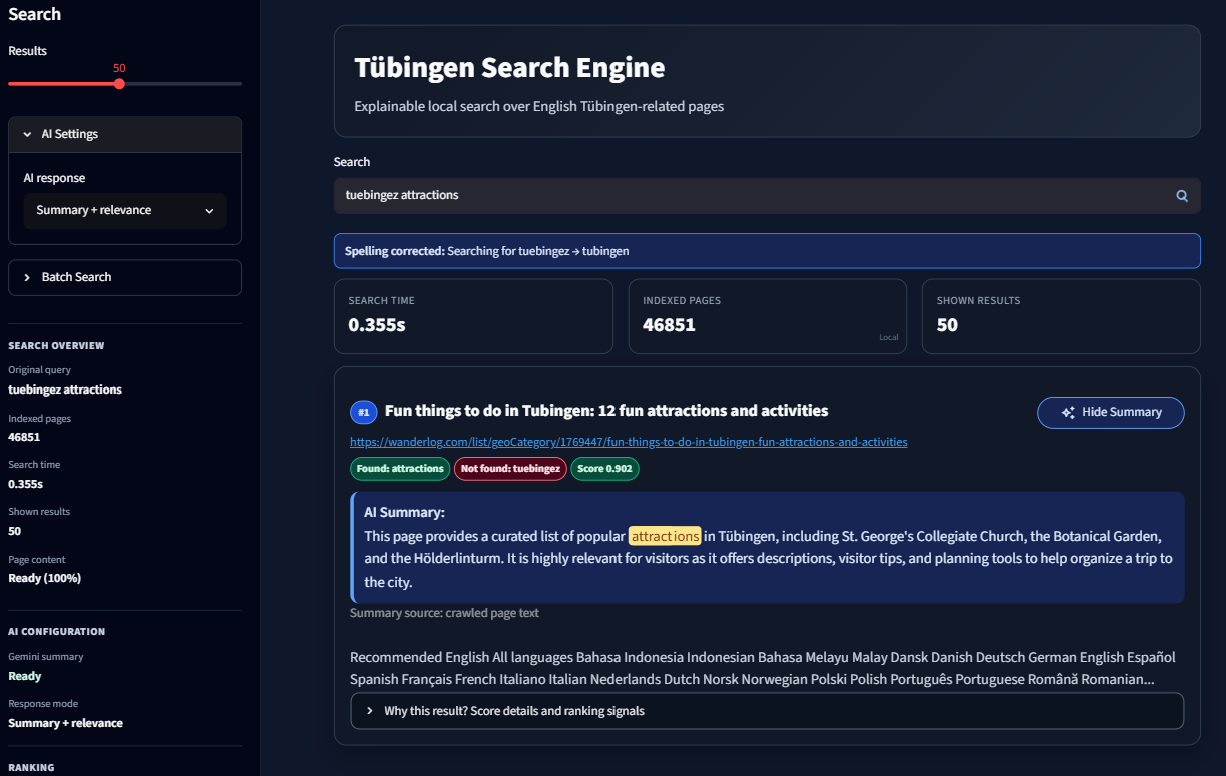
\includegraphics[height=55mm]{img/frontend.png}\hfill
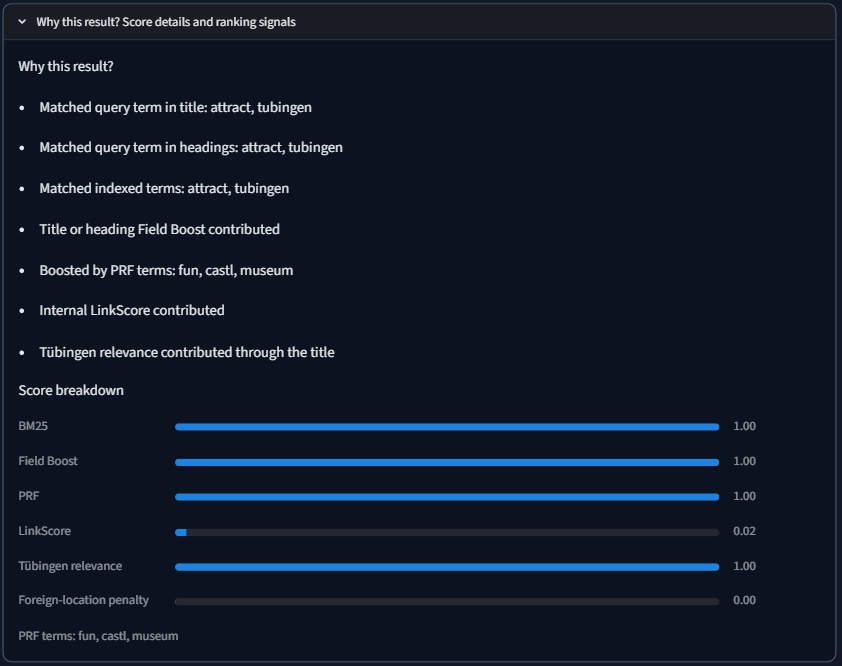
\includegraphics[height=55mm]{img/frontend-insights.png}\\[3pt]
{\small\textbf{Figure 1.} Search interface showing spelling correction, Found and Not found query-term badges, and an AI-generated result summary (left), and the expanded ranking explanation with its score breakdown (right).}
\end{center}

\subsection{Interactive interface}

\textbf{AI summaries.} Each result card has an \emph{AI Summary} button backed by
the Gemini API. \emph{Summary + relevance} connects the page summary to the query,
\emph{Summary only} gives a neutral overview, and \emph{Custom focus} accepts a short
user prompt, for example about opening hours or entrance fees. A custom animation is 
shown during AI generation. The summaries use cached page content, meaning the crawled
body text from the raw-page data; this content is not used for retrieval or ranking.
When unavailable, the snippet is used,
and if the available text is too short, the page can be fetched live. If Gemini is
unavailable or not configured, a local extractive summary is shown instead. Summaries
are cached to avoid unnecessary API calls.

\textbf{Explainable ranking.} Each result card directly shows its final ranking score.
A \emph{Found} badge lists the exact matched query terms, while \emph{Not found} lists
the remaining terms. Applied spelling corrections are shown above the results so users
know which terms were used for retrieval. For further detail, the expandable
\emph{Why this result?} view shows textual match evidence and a normalized breakdown
of every active component: BM25, Field Boost, PRF, LinkScore, T\"ubingen relevance and
foreign-location penalty.

\textbf{Controls and fallback modes.} Users can select between 5 and 100 displayed
results. The sidebar shows search time, index size, active ranking components, data
source (Supabase or local), Gemini status (ready or not configured), and page-content
loading progress (crawled body text for AI summaries). The interface accepts batch-file
uploads and returns the retrieved results as a downloadable \texttt{results.tsv}. Runtime
data normally comes from
a private Supabase bucket. Starting with \texttt{--local} disables Supabase, and
local index files provide a fallback if Supabase cannot be used. These options keep the
service reliable: if one feature or external service fails, the rest of the search
continues to work so the user notices as little of the failure as possible.

\subsection{Hosting and resource management}

When a user opens the hosted version, DuckDNS resolves the domain to the public IP of
the Oracle VM. Nginx, the reverse proxy, forwards the browser request to Streamlit on
the same VM. At startup, Streamlit downloads the compressed index and raw-page shards
from Supabase Storage, caches the index in RAM, and loads raw-page content gradually
for AI summaries. It reuses the cached index for retrieval and sends summary requests
to Gemini. The API key stays on the server; local use requires a separate key.

\textbf{Index caching.} Caching the loaded index was our largest runtime improvement:
it remains in RAM across Streamlit reruns and is reused for all searches. This reduced
search times from about ten seconds to usually below one second.

\textbf{Startup memory.} As the data grew, combining downloaded shards in RAM caused a
large startup peak. To avoid this, downloaded shards are streamed to a disk cache instead
of being combined in RAM. The index is then loaded into RAM and cached, so users can search
as soon as it is ready. Page content, which is only needed for AI summaries, is processed
gradually in the background. Loading all raw pages therefore takes longer, but this avoids
the RAM peak and improves scalability.

\newpage
\begin{thebibliography}{9}

\bibitem{robertson2009bm25}
Stephen Robertson and Hugo Zaragoza.
\textit{The Probabilistic Relevance Framework: BM25 and Beyond}.
Foundations and Trends in Information Retrieval,
3(4):333--389, 2009.

\bibitem{levenshtein1966}
Vladimir I. Levenshtein.
\textit{Binary Codes Capable of Correcting Deletions, Insertions and Reversals}.
Soviet Physics Doklady,
10(8):707--710, 1966.

\bibitem{streamlit}
Streamlit Inc.
Streamlit Documentation.
\url{https://docs.streamlit.io/}.
Accessed: August 5, 2026.

\bibitem{oracleCompute}
Oracle Corporation.
Oracle Cloud
\url{https://docs.oracle.com/}.
Accessed: August 5, 2026.

\bibitem{supabaseStorage}
Supabase.
\textit{Storage}.
\url{https://supabase.com/docs/guides/storage}.
Accessed: August 5, 2026.

\end{thebibliography}

\end{document}